%%%%%%%%%%%%%%%%%%%%%%%%%%%%%%%%%%%%%%%%%%%%%%%%%%%%%%%%%%%%%%%
%
% Welcome to Overleaf --- just edit your LaTeX on the left,
% and we'll compile it for you on the right. If you open the
% 'Share' menu, you can invite other users to edit at the same
% time. See www.overleaf.com/learn for more info. Enjoy!
%
%%%%%%%%%%%%%%%%%%%%%%%%%%%%%%%%%%%%%%%%%%%%%%%%%%%%%%%%%%%%%%%
\documentclass[12pt, letterpaper]{article}
\title{This is My First \LaTeX\ Document}
\author{Pizofreude\thanks{Self-funded by [Pizofreude](https://ko-fi.com/pizofreude).}}
\date{January 2020}
\usepackage{graphicx} % Package for inserting image
\graphicspath{{images/}} % Args for image filepath
\usepackage{hyperref} % Package for inserting Markdown-like hyperlinks
\usepackage{listings} % Package for alternative method of WYSIWYG LaTeX syntax by ignoring its command.
\usepackage{amsmath} % For the equation* environment

\begin{document}

\maketitle

\newpage
\tableofcontents
\newpage

\section{Quick Introduction}

First document. This is a simple example, with no 
extra parameters or packages included.

This is second paragraph. A bit short but no body is perfect and I am nobody.

This is the third paragraph that I wrote wholeheartedly without much thought or in fact any thought at all.

There are currently Title, Author, and Date in this first \LaTeX document!

% This line is a comment and will not be typeset in this document. Best of all, the VS Code hotkey for commenting Ctrl+/ works as well!!! Still a commment.
Not a comment anymore, and now we know \% indicates comment in \LaTeX.

Just as I thought, new line or paragraph will end the comment command. Great and very intuitive!

This is how to \textbf{bold}, \textit{italic}, and \underline{underline} text in \LaTeX. We can combine it to our heart contents.

For example this is how to \textbf{\textit{\underline{bold, italic, and underline}}} text all at once!

\emph{Emphasis} is another great text format. If used in \emph{normal text}, it will \emph{italicized} it. If used in \textbf{\emph{bold text}}, it will \textbf{\emph{bold and italicized it}}. If used in \textit{italic text}, it will present it as \textit{\emph{normal text}}.

Note: some packages, such as Beamer, change the behaviour of the \textbackslash emph command. We can use \textbackslash\ to avoid escape character. E.g. \&, \{ and \} as well as at the end of \textbackslash\ to introduce space afterwards.

\section{Adding Image}

You need to upload images to your Overleaf project first before embedding it.
\textbackslash usepackage\{graphicx\}: \LaTeX package to import graphics in preamble.
\textbackslash graphicspath\{\{images/\}\}: In preamble, it configures the graphicx package filepath. It is recommended to create a directory name images in the working directory.
\textbackslash includegraphi- cs \{imageName\}: In body. it loads the imageName. Although the full file name, including its extension, is allowed in the \textbackslash includegraphics command, it’s considered best practice to omit the file extension because it will prompt LATEX to search for all the supported formats. Here's an example an image by uploading it from local machine to Overleaf:

\begin{figure}
    \centering
    
\includegraphics[scale=0.25]{images/hex.png}
    \caption{Hex logo.}
    \label{fig:Hex label}
\end{figure}

Generally, the graphic’s file name should not contain white spaces or multiple dots; it is also recommended to use lowercase letters for the file extension when uploading image files to Overleaf. Usage of camelCase for imageName is also recommended. Here's another example of image by URL:

\begin{figure}
    \centering
    \includegraphics[scale=0.3]{pulsex}
    \caption{PulseX logo.}
    \label{fig:PulseX Label}
\end{figure}

Another method of adding image amongst other options is inserting an image with cross-reference in the paragraph completed with page number where it is positioned. As you can see in Figure \ref{fig:Pulsechain logo.} and this image can be found on page \pageref{fig:Pulsechain logo.}.

\begin{figure}[h]
    \centering
    
\includegraphics[width=0.5\textwidth]{PulseChain}
    \caption{Pulsechain logo.}
    \label{fig:Pulsechain logo.}
\end{figure}

There are several noteworthy commands in the example:

\textbackslash includegraphics\[width=0.5\textbackslash textwidth\]\{PulseChain\}: This form of \textbackslash includegraphics instructs \LaTeX to set the figure’s width to 50\% of the text width—whose value is stored in the \textbackslash textwidth command.

\textbackslash caption\{Pulsechain logo.\}: As its name suggests, this command sets the figure caption which can be placed above or below the figure. If you create a list of figures this caption will be used in that list.

\textbackslash label\{fig:Pulsechain logo.\}: To reference this image within your document you give it a label using the \textbackslash label command. The label is used to generate a number for the image and, combined with the next command, will allow you to reference it.

\textbackslash ref\{fig:Pulsechain logo.\}: This code will be substituted by the number corresponding to the referenced figure.

Images incorporated in a \LaTeX document should be placed inside a figure environment, or similar, so that \LaTeX  can automatically position the image at a suitable location in your document.

Further guidance is contained in the following Overleaf help articles \href{https://www.overleaf.com/learn/latex/Positioning_of_Figures}{Positioning of Figures} and
 \href{https://www.overleaf.com/learn/latex/Inserting_Images}{Inserting Images}.

 \section{Creating lists in \LaTeX}

You can create different types of list using \textit{environments}, which are used to encapsulate the \LaTeX code required to implement a specific typesetting feature. An \textit{environments} starts with \textbackslash begin{environment-name} and ends with \textbackslash end{environment-name} where \textit{environment-name} might be figure, tabular or one of the list types: \textbf{itemize} for unordered lists or \textbf{enumerate} for ordered lists.

\subsection{Unordered lists}

\begin{verbatim} % The verbatim environment is used to write LaTeX syntax without
processing it.
\begin{itemize}
  \item The individual entries are indicated with a black dot, a
  so-called bullet.
  \item The text in the entries may be of any length.
\end{itemize}
\end{verbatim}

The output will be as follows:

\begin{itemize}
  \item The individual entries are indicated with a black dot, a so-called bullet.
  \item The text in the entries may be of any length.
\end{itemize}

\subsection{Ordered lists}

Ordered lists use the same syntax as unordered lists but are created using the enumerate environment:

\begin{verbatim}
\begin{enumerate}
  \item This is the first entry in our list.
  \item The list numbers increase with each entry we add.
\end{enumerate}
\end{verbatim}

The output will be:

\begin{enumerate}
  \item This is the first entry in our list.
  \item The list numbers increase with each entry we add.
\end{enumerate}

As with unordered lists, each entry must be preceded by the \textbackslash item command which, here, automatically generates the numeric ordered-list label value, starting at 1. For further information, refer to:

\begin{itemize}
    \item \href{https://www.overleaf.com/project/new/template/25521?id=107987258&templateName=Demonstrating+various+types+of+LaTeX+list&latexEngine=pdflatex&texImage=texlive-full%3A2022.1&mainFile=}{Demonstrating various types of LaTeX list}
    \item \href{https://www.overleaf.com/learn/latex/Lists}{Comprehensive List Styles in \LaTeX}
\end{itemize}

\section{Writing Code Syntax in \LaTeX}

\textit{Inline code} for \LaTeX syntax with \textbf{WYSIWYG} method can be achieved by using \textbackslash textbackslash command. For \textit{code block}, we can use the \textit{verbatim environment} to write \LaTeX syntax as a \textit{code block} in \LaTeX and ignore the \LaTeX commands. The \textit{verbatim environment} is used to display text exactly as it is written, without interpreting any \LaTeX commands.

Here's an example of how to use the verbatim environment:

\begin{verbatim}
\begin{verbatim}
This is an example of the verbatim environment.
It can be used to display LaTeX code without interpreting any
commands.
For example, \textbf{this} will not be bold.
\\end {verbatim}
\end{verbatim}

Alternatively, you can also use the \textit{lstlisting environment} provided by the \textit{listings package}, which is a powerful package for typesetting source code in \LaTeX documents. It has many options for customization, including syntax highlighting. User can import \textbackslash usepackage\{listings\} in the \textbf{preamble}.

\begin{verbatim}
\begin{lstlisting}[language=TeX]
This is an example of the lstlisting environment.
It can also be used to display LaTeX code without interpreting
any commands.
For example, \textbf{this} will not be bold.
\end{lstlisting}
\end{verbatim}

The output will be:

\begin{lstlisting}[language=TeX]
This is an example of the lstlisting environment.
It can also be used to display LaTeX code without inter-
preting any commands.
For example, \textbf{this} will not be bold.
\end{lstlisting}

\subsection{Code Block for Other Programming \& Tech Languages}

User can include many other programming languages as well as tech languages such as Markdown and etc pp. We can use bash language as alternative to \textit{verbatim environment} and \textit{lstlisting environment} which looks more professional as well.
Refer to these lists for further information:

\begin{enumerate}
    \item \href{https://www.overleaf.com/learn/latex/Code_listing}{Code Listing in \LaTeX}
    \item \href{https://www.overleaf.com/learn/latex/Code_Highlighting_with_minted}{Code Highlighting with \textit{minted environment}}
\end{enumerate}

\section{Adding math to \LaTeX}

One of the main advantages of \LaTeX is the ease with which mathematical expressions can be written. \LaTeX provides two writing modes for typesetting mathematics:

\textit{inline math} mode used for writing formulas that are part of a paragraph
\textit{display math} mode used to write expressions that are not part of a text or paragraph and are typeset on separate lines.

\subsection{Inline Math Mode}

Here's an example of how to write inline math:

\begin{verbatim}
\documentclass[12pt, letterpaper]{article}
\begin{document}
In physics, the mass-energy equivalence is stated 
by the equation $E=mc^2$, discovered in 1905 by Albert Einstein.
\end{document}    
\end{verbatim}

The output will be:

In physics, the mass-energy equivalence is stated 
by the equation $E=mc^2$, discovered in 1905 by Albert Einstein. $Inline Math Formula$.

To typeset inline-mode math you can use one of these delimiter pairs: \textbackslash( ... \textbackslash), \$ ... \$ or \textbackslash begin\{math\} ... \textbackslash end\{math\}, as demonstrated in the following example:

\begin{verbatim}
\begin{math}
E=mc^2
\end{math} is typeset in a paragraph using inline math mode---as
is $E=mc^2$, and so too is \(E=mc^2\).
\end{verbatim}

and the output is:

\begin{math}
E=mc^2
\end{math} is typeset in a paragraph using inline math mode---as is $E=mc^2$, and so too is \(E=mc^2\).

\subsection{Display math mode}

Equations typeset in display mode can be numbered or unnumbered, as in the following example:

\begin{verbatim}
\documentclass[12pt, letterpaper]{article}
\begin{document}
The mass-energy equivalence is described by the famous equation
\[ E=mc^2 \] discovered in 1905 by Albert Einstein. 

In natural units ($c = 1$), the formula expresses the identity
\begin{equation}
E=m
\end{equation}
\end{document}
\end{verbatim}

and the output:

The mass-energy equivalence is described by the famous equation
\[ E=mc^2 \] discovered in 1905 by Albert Einstein. 

In natural units ($c = 1$), the formula expresses the identity
\begin{equation}
E=m
\end{equation}

To typeset display-mode math you can use one of these delimiter pairs: \textbackslash[ ... \textbackslash], \textbackslash begin\{displaymath\} ... \textbackslash end\{displaymath\} or \textbackslash begin\{equation\} ... \textbackslash end\{equation\}. Historically, typesetting display-mode math required use of \$\$ characters delimiters, as in \$\$ ... display math here ...\$\$, but this method is no longer recommended: use \LaTeX’s delimiters \textbackslash[ ... \textbackslash] instead.

\subsection{More Math Examples}

This subsection demonstrates more range of mathematical content typeset using \LaTeX.

\begin{verbatim}
\documentclass{article}
\begin{document}
Subscripts in math mode are written as $a_b$ and superscripts 
are written as $a^b$. These can be combined and nested to write 
expressions such as

\[ T^{i_1 i_2 \dots i_p}_{j_1 j_2 \dots j_q} = T(x^{i_1},\dots,
x^{i_p},e_{j_1},\dots,e_{j_q}) \]
 
We write integrals using $\int$ and fractions using $\frac{a}{b}$.
Limits are placed on integrals using superscripts and subscripts:

\[ \int_0^1 \frac{dx}{e^x} =  \frac{e-1}{e} \]

Lower case Greek letters are written as $\omega$ $\delta$ etc.
while upper case Greek letters are written as $\Omega$ $\Delta$.

Mathematical operators are prefixed with a backslash as 
$\sin(\beta)$, $\cos(\alpha)$, $\log(x)$ etc.
\end{document}
\end{verbatim}

 These produce the output:

 Subscripts in math mode are written as $a_b$ and superscripts are written as $a^b$. These can be combined and nested to write expressions such as

\[ T^{i_1 i_2 \dots i_p}_{j_1 j_2 \dots j_q} = T(x^{i_1},\dots,x^{i_p},e_{j_1},\dots,e_{j_q}) \]

or

\begin{equation}
    T^{i_1 i_2 \dots i_p}_{j_1 j_2 \dots j_q} = T(x^{i_1},\dots,x^{i_p},e_{j_1},\dots,e_{j_q})
\end{equation}
 
We write integrals using $\int$ and fractions using $\frac{a}{b}$. Limits are placed on integrals using superscripts and subscripts:

\[ \int_0^1 \frac{dx}{e^x} =  \frac{e-1}{e} \]

or

\begin{equation}
    \int_0^1 \frac{dx}{e^x} =  \frac{e-1}{e}
\end{equation}

Lower case Greek letters are written as $\omega$ $\delta$ etc. while upper case Greek letters are written as $\Omega$ $\Delta$.

Mathematical operators are prefixed with a backslash as $\sin(\beta)$, $\cos(\alpha)$, $\log(x)$ etc.

The next example uses the equation* environment which is provided by the amsmath package, so we need to add the following line to our document preamble:

\begin{verbatim}
    \usepackage{amsmath}% For the equation* environment
\end{verbatim}

For further information on using amsmath see the \href{https://www.overleaf.com/learn/latex/Aligning_equations}{help article}.

\begin{verbatim}
\documentclass{article}
\usepackage{amsmath}% For the equation* environment
\begin{document}
\section{First example}

The well-known Pythagorean theorem \(x^2 + y^2 = z^2\) was proved 
to be invalid for other exponents, meaning the next equation has 
no integer solutions for \(n>2\):

\[ x^n + y^n = z^n \]

\section{Second example}

This is a simple math expression \(\sqrt{x^2+1}\) inside text. 
And this is also the same: 
\begin{math}
\sqrt{x^2+1}
\end{math}
but by using another command.

This is a simple math expression without numbering
\[\sqrt{x^2+1}\] 
separated from text.

This is also the same:
\begin{displaymath}
\sqrt{x^2+1}
\end{displaymath}

\ldots and this:
\begin{equation*}
\sqrt{x^2+1}
\end{equation*}
\\end{document}
\end{verbatim}

which outputs:

\subsubsection{First example}

The well-known Pythagorean theorem \(x^2 + y^2 = z^2\) was proved to be invalid for other exponents, meaning the next equation has no integer solutions for \(n>2\):

\[ x^n + y^n = z^n \]

\subsubsection{Second example}

This is a simple math expression \(\sqrt{x^2+1}\) inside text. 
And this is also the same: 
\begin{math}
\sqrt{x^2+1}
\end{math}
but by using another command.

This is a simple math expression without numbering
\[\sqrt{x^2+1}\] 
separated from text.

This is also the same:
\begin{displaymath}
\sqrt{x^2+1}
\end{displaymath}

\ldots and this:
\begin{equation*}
\sqrt{x^2+1}
\end{equation*}

The possibilities with math in \LaTeX are endless so be sure to visit the help pages for advice and more examples on specific topics:

\begin{itemize}
    \item \href{https://www.overleaf.com/learn/latex/Mathematical_expressions}{Mathematical expressions}
    \item \href{https://www.overleaf.com/learn/latex/Subscripts_and_superscripts}{Subscripts and superscripts}
    \item \href{https://www.overleaf.com/learn/latex/Brackets_and_Parentheses}{Brackets and Parentheses}
    \item \href{https://www.overleaf.com/learn/latex/Fractions_and_Binomials}{Fractions and Binomials}
    \item \href{https://www.overleaf.com/learn/latex/Aligning_equations_with_amsmath}{Aligning Equations}
    \item \href{https://www.overleaf.com/learn/latex/Operators}{Operators}
    \item \href{https://www.overleaf.com/learn/latex/Spacing_in_math_mode}{Spacing in math mode}
    \item \href{https://www.overleaf.com/learn/latex/Integrals%2C_sums_and_limits}{Integrals, sums and limits}
    \item \href{https://www.overleaf.com/learn/latex/Display_style_in_math_mode}{Display style in math mode}
    \item \href{https://www.overleaf.com/learn/latex/List_of_Greek_letters_and_math_symbols}{List of Greek letters and math symbols}
    \item \href{https://www.overleaf.com/learn/latex/Mathematical_fonts}{Mathematical fonts}
\end{itemize}

\section{Basic document structure}

Next, we explore abstracts and how to partition a \LaTeX document into different chapters, sections and paragraphs.

\subsection{Abstracts}

Scientific articles usually provide an abstract which is a brief overview/summary of their core topics, or arguments. The next example demonstrates typesetting an abstract using \LaTeX’s abstract environment:

\begin{verbatim}
\documentclass{article}
\begin{document}
\begin{abstract}
This is a simple paragraph at the beginning of the 
document. A brief introduction about the main subject.
\end{abstract}
\end{document}
\end{verbatim}

This example produces the following output:

\begin{abstract}
This is a simple paragraph at the beginning of the 
document. A brief introduction about the main subject.
\end{abstract}

\subsection{Paragraphs and new lines}

With the abstract in place, we can begin writing our first paragraph. The next example demonstrates:

how a new paragraph is created by pressing the "enter" key twice, ending the current line and inserting a subsequent blank line;
how to start a new line without starting a new paragraph by inserting a manual line break using the \textbackslash \textbackslash\ command, which is a double backslash; alternatively, use the \textbackslash newline command.
The third paragraph in this example demonstrates use of the commands \textbackslash \textbackslash\ and \textbackslash newline:

\begin{verbatim}
\documentclass{article}
\begin{document}

\begin{abstract}
This is a simple paragraph at the beginning of the 
document. A brief introduction about the main subject.
\end{abstract}

After our abstract we can begin the first paragraph, then press 
''enter'' twice to start the second one.

This line will start a second paragraph.

I will start the third paragraph and then add \\ a manual line
break which causes this text to start on a new line but remains
part of the same paragraph. Alternatively, I can use the \verb|
\newline|\newline command to start a new line, which is also
part of the same paragraph.
\end{document}
\end{verbatim}

which outputs:

\begin{abstract}
This is a simple paragraph at the beginning of the 
document. A brief introduction about the main subject.
\end{abstract}

After our abstract we can begin the first paragraph, then press ``enter'' twice to start the second one.

This line will start a second paragraph.

I will start the third paragraph and then add \\ a manual line break which causes this text to start on a new line but remains part of the same paragraph. Alternatively, I can use the \verb|\newline|\newline command to start a new line, which is also part of the same paragraph.

Note how \LaTeX automatically indents paragraphs—except immediately after document headings such as section and subsection—\href{https://www.overleaf.com/learn/latex/Learn_LaTeX_in_30_minutes#Chapters_and_sections}{as we see here.}

New users are advised that multiple \textbackslash \textbackslash or \textbackslash newlines should not used to “simulate” paragraphs with larger spacing between them because this can interfere with \LaTeX’s typesetting algorithms. The recommended method is to continue using blank lines for creating new paragraphs, without any \textbackslash \textbackslash, and load the \href{https://ctan.org/pkg/parskip?lang=en}{parskip package} by adding \textbackslash usepackage\{parskip\} to the preamble.

Further information on paragraphs can be found in the following articles:

\begin{itemize}
    \item \href{https://www.overleaf.com/learn/latex/Paragraphs_and_new_lines}{Paragraphs and new lines}
    \item \href{https://www.overleaf.com/learn/latex/Articles/How_to_change_paragraph_spacing_in_LaTeX}{How to change paragraph spacing in LaTeX}
    \item \href{https://www.overleaf.com/learn/latex/Errors/LaTeX_Error%3A_There%27s_no_line_here_to_end}{LaTeX Error: There's no line here to end provides additional advice and guidance on using \textbackslash \textbackslash.}
\end{itemize}

\subsection{Chapters and sections}

Longer documents, irrespective of authoring software, are usually partitioned into parts, chapters, sections, subsections and so forth. \LaTeX also provides document-structuring commands but the available commands, and their implementations (what they do), can depend on the document class being used. By way of example, documents created using the book class can be split into parts, chapters, sections, subsections and so forth but the letter class does not provide (support) any commands to do that.

This next example demonstrates commands used to structure a document based on the book class:

\begin{verbatim}
\documentclass{book}
\begin{document}

\chapter{First Chapter}

\section{Introduction}

This is the first section.

Lorem  ipsum  dolor  sit  amet,  consectetuer  adipiscing  
elit. Etiam  lobortisfacilisis sem.  Nullam nec mi et 
neque pharetra sollicitudin.  Praesent imperdietmi nec ante. 
Donec ullamcorper, felis non sodales...

\section{Second Section}

Lorem ipsum dolor sit amet, consectetuer adipiscing elit.  
Etiam lobortis facilisissem.  Nullam nec mi et neque pharetra 
sollicitudin.  Praesent imperdiet mi necante...

\subsection{First Subsection}
Praesent imperdietmi nec ante. Donec ullamcorper, felis non 
sodales...

\section*{Unnumbered Section}
Lorem ipsum dolor sit amet, consectetuer adipiscing elit.  
Etiam lobortis facilisissem...
\\end{document}
\end{verbatim}

This example produces the following output:

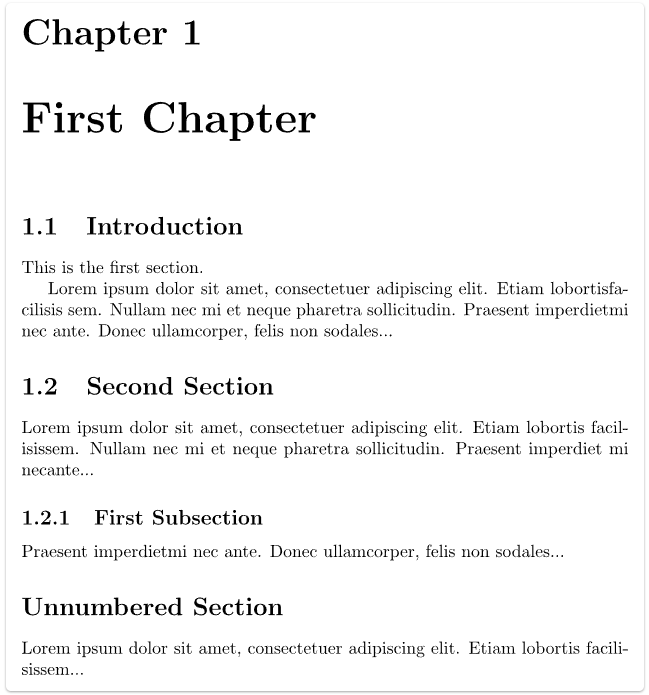
\includegraphics[scale=0.7]{brave_C1X0ompXxZ}

The names of sectioning commands are mostly self-explanatory; for example, \textbackslash chapter\{First Chapter\} creates a new chapter titled First Chapter, \textbackslash section\{Introduction\} produces a section titled Introduction, and so forth. Sections can be further divided into \textbackslash subsection\{...\} and even \textbackslash subsubsection\{...\}. The numbering of sections, subsections etc. is automatic but can be disabled by using the so-called starred version of the appropriate command which has an asterisk (*) at the end, such as \textbackslash section*\{...\} and \textbackslash subsection*\{...\}.

Collectively, \LaTeX document classes provide the following sectioning commands, with specific classes each supporting a relevant subset:

\begin{verbatim}
\part{part}
\chapter{chapter}
\section{section}
\subsection{subsection}
\subsubsection{subsubsection}
\paragraph{paragraph}
\subparagraph{subparagraph}
\end{verbatim}

In particular, the \textbackslash part and \textbackslash chapter commands are only available in the report and book document classes. For more information about document structure commands, feel free to visit \href{https://www.overleaf.com/learn/latex/Sections_and_chapters}{article about sections and chapters}.

\section{Creating tables}

The following examples show how to create tables in \LaTeX, including the addition of lines (rules) and captions.

\subsection{Creating a basic table in \LaTeX}

We start with an example showing how to typeset a basic table:

\begin{verbatim}
\begin{center}
\begin{tabular}{c c c}
 cell1 & cell2 & cell3 \\ 
 cell4 & cell5 & cell6 \\  
 cell7 & cell8 & cell9    
\end{tabular}
\end{center}
\end{verbatim}

which produces:

\begin{center}
\begin{tabular}{c c c}
 cell1 & cell2 & cell3 \\ 
 cell4 & cell5 & cell6 \\  
 cell7 & cell8 & cell9    
\end{tabular}
\end{center}

The tabular environment is the default \LaTeX method to create tables. You must specify a parameter to this environment, in this case \{c c c\} which advises \LaTeX that there will be three columns and the text inside each one must be centred. You can also use r to right-align the text and l to left-align it. The alignment symbol \& is used to demarcate individual table cells within a table row. To end a table row use the new line command \textbackslash\textbackslash. Our table is contained within a center environment to make it centred within the text width of the page.

\subsection{Adding borders}

The tabular environment supports horizontal and vertical lines (rules) as part of the table:

to add horizontal rules, above and below rows, use the \textbackslash hline command
to add vertical rules, between columns, use the vertical line parameter |
In this example the argument is {|c|c|c|} which declares three (centred) columns each separated by a vertical line (rule); in addition, we use \textbackslash hline to place a horizontal rule above the first row and below the final row:

\begin{verbatim}
\begin{center}
\begin{tabular}{|c|c|c|} 
 \hline
 cell1 & cell2 & cell3 \\ 
 cell4 & cell5 & cell6 \\ 
 cell7 & cell8 & cell9 \\ 
 \hline
\end{tabular}
\end{center}
\end{verbatim}

The output is:

\begin{center}
\begin{tabular}{|c|c|c|} 
 \hline
 cell1 & cell2 & cell3 \\ 
 cell4 & cell5 & cell6 \\ 
 cell7 & cell8 & cell9 \\ 
 \hline
\end{tabular}
\end{center}

Here is a further example:

\begin{verbatim}
\begin{center}
 \begin{tabular}{||c c c c||} 
 \hline
 Col1 & Col2 & Col2 & Col3 \\ [0.5ex] 
 \hline\hline
 1 & 6 & 87837 & 787 \\ 
 \hline
 2 & 7 & 78 & 5415 \\
 \hline
 3 & 545 & 778 & 7507 \\
 \hline
 4 & 545 & 18744 & 7560 \\
 \hline
 5 & 88 & 788 & 6344 \\ [1ex] 
 \hline
\end{tabular}
\end{center}
\end{verbatim}


which output:

\begin{center}
 \begin{tabular}{||c c c c||} 
 \hline
 Col1 & Col2 & Col2 & Col3 \\ [0.5ex] 
 \hline\hline
 1 & 6 & 87837 & 787 \\ 
 \hline
 2 & 7 & 78 & 5415 \\
 \hline
 3 & 545 & 778 & 7507 \\
 \hline
 4 & 545 & 18744 & 7560 \\
 \hline
 5 & 88 & 788 & 6344 \\ [1ex] 
 \hline
\end{tabular}
\end{center}

Tip!

Creating tables in \LaTeX can be time-consuming so you may want to use the \href{TablesGenerator.com}{TablesGenerator.com} online tool to export \LaTeX code for tabulars.

\subsection{Captions, Labels and References}

You can caption and reference tables in much the same way as images. The only difference is that instead of the figure environment, you use the table environment.

\begin{verbatim}
Table \ref{table:data} shows how to add a table caption and reference a table.
\begin{table}[h!]
\centering
\begin{tabular}{||c c c c||} 
 \hline
 Col1 & Col2 & Col2 & Col3 \\ [0.5ex] 
 \hline\hline
 1 & 6 & 87837 & 787 \\ 
 2 & 7 & 78 & 5415 \\
 3 & 545 & 778 & 7507 \\
 4 & 545 & 18744 & 7560 \\
 5 & 88 & 788 & 6344 \\ [1ex] 
 \hline
\end{tabular}
\caption{Table to test captions and labels.}
\label{table:data}
\end{table}
\end{verbatim}

The output is:

Table \ref{table:data} shows how to add a table caption and reference a table.
\begin{table}[h!]
\centering
\begin{tabular}{||c c c c||} 
 \hline
 Col1 & Col2 & Col2 & Col3 \\ [0.5ex] 
 \hline\hline
 1 & 6 & 87837 & 787 \\ 
 2 & 7 & 78 & 5415 \\
 3 & 545 & 778 & 7507 \\
 4 & 545 & 18744 & 7560 \\
 5 & 88 & 788 & 6344 \\ [1ex] 
 \hline
\end{tabular}
\caption{Table to test captions and labels.}
\label{table:data}
\end{table}

\section{Adding a Table of Contents}

Creating a table of contents is straightforward because the command \textbackslash tableofcontents does almost all the work for you:

\begin{verbatim}
\documentclass{article}
\title{Sections and Chapters}
\author{Gubert Farnsworth}
\date{August 2022}
\begin{document}
  
\maketitle
  
\tableofcontents

\section{Introduction}
   
This is the first section.
      
Lorem  ipsum  dolor  sit  amet,  consectetuer  adipiscing  
elit.   Etiam  lobortisfacilisis sem.  Nullam nec mi et 
neque pharetra sollicitudin.  Praesent imperdietmi nec ante. 
Donec ullamcorper, felis non sodales...
       
\section*{Unnumbered Section}
\addcontentsline{toc}{section}{Unnumbered Section}

Lorem ipsum dolor sit amet, consectetuer adipiscing elit.  
Etiam lobortis facilisissem.  Nullam nec mi et neque pharetra 
sollicitudin.  Praesent imperdiet mi necante...

\section{Second Section}
       
Lorem ipsum dolor sit amet, consectetuer adipiscing elit.  
Etiam lobortis facilisissem.  Nullam nec mi et neque pharetra 
sollicitudin.  Praesent imperdiet mi necante...
\end{document}
\end{verbatim}

with the output as seen in this document's TOC after \textbackslash maketitle command.

Sections, subsections and chapters are automatically included in the table of contents. To manually add entries, such as an unnumbered section, use the command \textbackslash addcontentsline as shown in the commandline example above.

\section{Finding and Using \LaTeX Packages}

\LaTeX not only delivers significant typesetting capabilities but also provides a framework for extensibility through the use of add-on packages. Rather than attempting to provide commands and features that “try to do everything”, \LaTeX is designed to be extensible, allowing users to load external bodies of code (packages) that provide more specialist typesetting capabilities or extend \LaTeX’s built-in features—such as typesetting tables. As observed in the section \href{https://www.overleaf.com/learn/latex/Learn_LaTeX_in_30_minutes#Adding_images}{Adding images}, the graphicx package extends \LaTeX by providing commands to import graphics files and was loaded (in the preamble) by writing \textbackslash usepackage\{graphicx\} command.

\subsection{Loading Packages}

As noted above, packages are loaded in the document preamble via the \textbackslash usepackage command but because (many) \LaTeX packages provide a set of options, which can be used to configure their behaviour, the \textbackslash usepackage command often looks like this:

\begin{verbatim}
\usepackage[options]{somepackage}
\end{verbatim}

The square brackets “[...]” inform \LaTeX which set of options should be applied when it loads somepackage. Within the set of options requested by the user, individual options, or settings, are typically separated by a comma; for example, the \href{https://ctan.org/pkg/geometry}{geometry package} provides many options to configure page layout in \LaTeX, so a typical use of geometry might look like this:

\begin{verbatim}
\usepackage[total={6.5in,8.75in},
top=1.2in, left=0.9in, includefoot]{geometry}
\end{verbatim}

The geometry package is one example of a package written and contributed by members of the global \LaTeX community and made available, for free, to anyone who wants to use it.

If a \LaTeX package does not provide any options, or the user wants to use the default values of a package’s options, it would be loaded like this:

\begin{verbatim}
\usepackage{somepackage}
\end{verbatim}

When you write \textbackslash usepackage[...]\{somepackage\} \LaTeX looks for a corresponding file called \textit{somepackage.sty}, which it needs to load and process—to make the package commands available and execute any other code provided by that package. If \LaTeX cannot find \textit{somepackage.sty} it will terminate with an error, as demonstrated in the following Overleaf example:

\begin{figure}
    \centering
    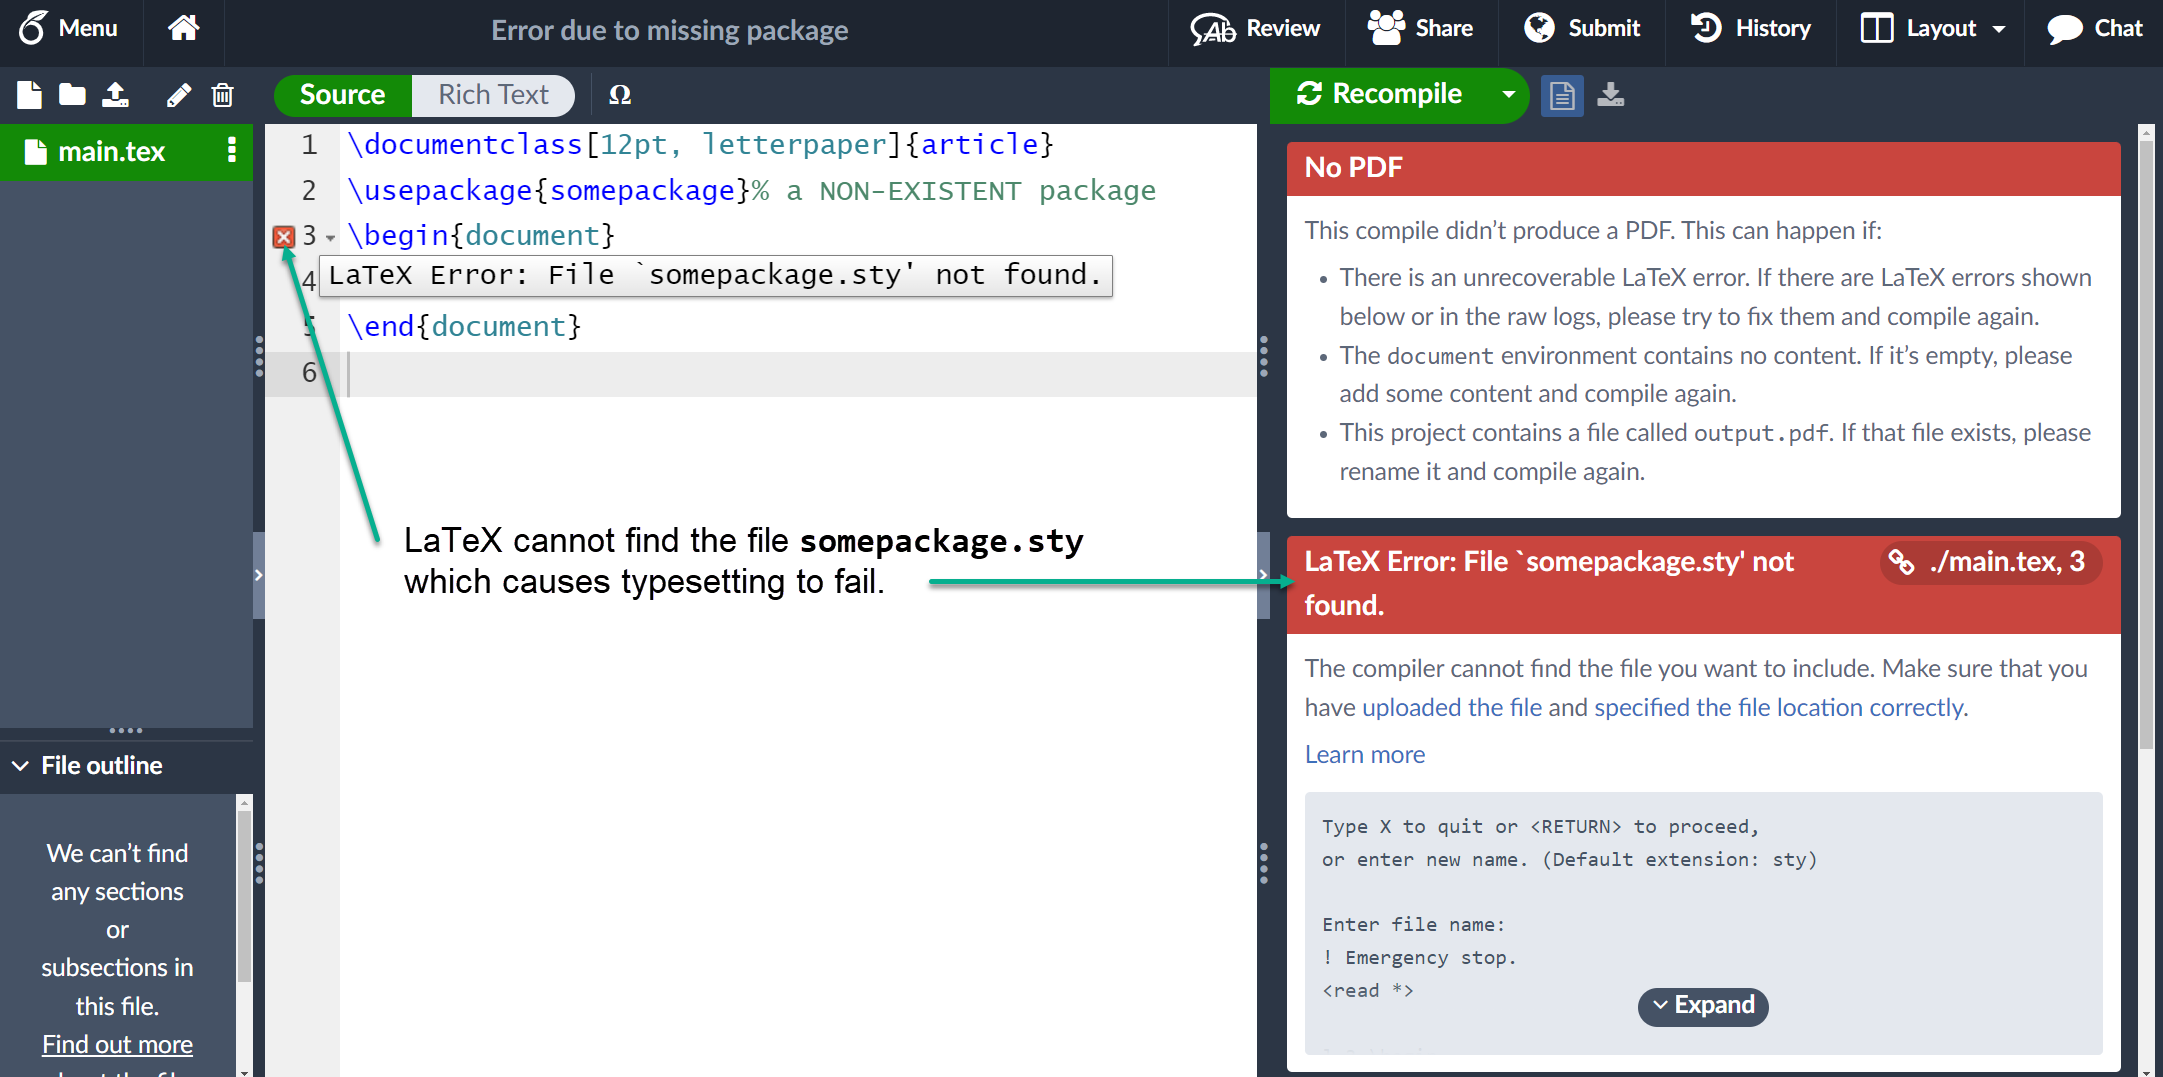
\includegraphics[scale=0.2]{images/LL30packagefail.png}
    \caption{Package fails to load.}
    \label{fig:Some package fail to load error.}
\end{figure}

\section{Finding Information about Packages: CTAN}

Packages are distributed through the \href{https://www.ctan.org/}{Comprehensive TeX Archive Network}, usually referred to as CTAN, which, at the time of writing, hosts 6287 packages from 2881 contributors. CTAN \href{https://www.ctan.org/ctan}{describes itself} as

\begin{quote}
    ... a set of Internet sites around the world that offer TEX-related material for download.
\end{quote}

You can browse CTAN to look for useful packages; for example:

\begin{itemize}
    \item \href{https://www.ctan.org/topics/cloud}{by topic}
    \item \href{https://www.ctan.org/pkg}{alphabetically} (useful if you know the package name)
    \item You can also use the \href{https://www.ctan.org/pkg}{search facility} (at the top of the page).
\end{itemize}

\newpage

\section*{Packages available on Overleaf: Introducing \TeX Live}
\addcontentsline{toc}{section}{Packages available on Overleaf: Introducing \TeX Live}

Once per year a (large) subset of packages hosted on CTAN, plus \LaTeX-related fonts and other software, is collated and distributed as a system called \href{https://tug.org/texlive/}{\TeX Live}, which can be used to install your own (local) \LaTeX setup. In fact,  \href{https://www.overleaf.com/learn/latex/Overleaf_and_TeX_Live}{Overleaf’s servers also use \TeX Live} and are updated when a new version of TeX Live is released. Overleaf’s \TeX Live updates are not immediate but take place a few months post-release, giving us time to perform compatibility tests of the new \TeX Live version with the thousands of \href{https://www.overleaf.com/gallery}{templates contained in our gallery}. For example, here is our \TeX Live 2020 upgrade \href{https://www.overleaf.com/blog/tex-live-2020-now-available}{announcement}.\\

Although \TeX Live contains a (large) subset of CTAN packages it is possible to find an interesting package, such as \href{https://ctan.org/pkg/igo?lang=en}{igo for typesetting Go diagrams}, which is hosted on CTAN but not included in (distributed by) \TeX Live and thus unavailable on Overleaf. Some packages hosted on CTAN are not part of \TeX Live due to a variety of reasons: perhaps a package is obsolete, has licensing problems, is extremely new (recently uploaded) or has platform dependencies, such as working on Windows but not Linux.\\

New packages, and updates to existing ones, are uploaded to CTAN all year round but updates to \TeX Live are distributed annually; consequently, packages contained in the current version of \TeX Live will not be as up-to-date as those hosted on CTAN. Because Overleaf’s servers use \TeX Live it is possible that packages installed on our servers—i.e., ones available to our users—might not be the very latest versions available on CTAN but, generally, this is unlikely to be problematic.

\end{document}
